\documentclass[11pt,a4paper]{article}

\usepackage[margin=2.4cm]{geometry}
\usepackage[T1]{fontenc}
\usepackage[utf8]{inputenc}
\usepackage{lmodern}
\usepackage{amsmath,amssymb,amsthm}
\usepackage{booktabs}
\usepackage{graphicx}
\usepackage{xcolor}
\usepackage[colorlinks=true,linkcolor=blue!50!black,citecolor=blue!50!black,urlcolor=blue!50!black]{hyperref}

\newcommand{\code}[1]{\texttt{\detokenize{#1}}}
\newcommand{\E}{\mathbb{E}}
\newcommand{\Var}{\operatorname{Var}}
\newcommand{\Cov}{\operatorname{Cov}}
\newcommand{\diag}{\operatorname{diag}}
\newcommand{\tr}{\operatorname{tr}}
\newcommand{\N}{\mathcal{N}}
\newcommand{\bfk}{\mathbf{k}}
\newtheorem{remark}{Remark}

\title{Deep variational Gaussian process networks in geoML:\\
the second moment, realizations that carry it,\\
and what the code does}
\author{Prepared for Ítalo Gomes Gonçalves \\ branch \code{deep-second-moment}, commits \code{c6d707c}--\code{1b84ed5}}
\date{19 October 2026}

\begin{document}
\sloppy
\maketitle

\begin{abstract}
geoML builds spatial models as networks of variational Gaussian process
(GP) nodes. A node whose input is another node's uncertain output --- a
deep layer, or a \code{GPWalk} --- reports moments that, until this work,
left out the spread of its mean over the input --- 16--61\% of the deep
model's variance on the folded section --- and its realizations carried
still less: 25--59\% of the variance they were reported with, 6\% on a
shallow GP with three experts. This
report sets out the theory of the node as geoML implements it (the
whitened variational posterior, the experts, the expected kernel), then
the three pieces added on the branch: (i)~the \emph{second moment} at
uncertain inducing inputs, by a quadrature over the input with the
inducing inputs conditioned on each node; (ii)~\emph{pathwise
realizations}, every expert drawing from one random-feature prior, with
Matheron's rule supplying what the inducing points leave out and an exact
rescale making the blend hold the reported variance; and (iii)~a
prediction that integrates the realizations' own residual analytically.
Each equation is tied to the function that computes it. The last sections
report the measurements: the gates, training on the folded section,
Walker Lake and chapter~16, two regressions traced to their commits, and
a profile of where the time goes.
\end{abstract}

\tableofcontents
\newpage

%=====================================================================
\section{The variational GP node}\label{sec:node}
%=====================================================================

\subsection{Kernel and inputs}

A GP node \code{BasicGP} reads coordinates $x\in\mathbb{R}^d$ from its
parent and models a latent function $f:\mathbb{R}^d\to\mathbb{R}^s$ ($s$
outputs, \code{size}) whose components are independent GPs with unit
variance and a common correlation $k$. Distances are measured in
\emph{ranges}: with $\rho_j$ the range of dimension $j$, the scaled
distance is $\delta^2=\sum_j (x_j-y_j)^2/\rho_j^2$. Every kernel the deep
machinery accepts is written as a positive mixture of Gaussians in
$\delta$ (\code{_kernel_components}):
\begin{equation}\label{eq:mixture}
  k(x,y) \;=\; c + \sum_{q=1}^{Q} w_q \exp\!\left(-\omega_q\,\delta^2\right),
  \qquad w_q>0,\; c\ge 0 .
\end{equation}
The Gaussian kernel is one component, $\omega_1=3$, $w_1=1$, so that the
range is the practical range ($k=e^{-3}$ at $\delta=1$). The Matérn family
and the exponential are tables of eight fitted Gaussians each
(\code{_KERNEL_MIXTURES}, weights summing to one, within $5\times10^{-4}$
of the exponential); the rational quadratic is 48 components placed about
its trained scale. Spherical and cubic kernels are not mixtures and are
refused where an input is uncertain.

\subsection{Inducing points and the whitened posterior}

The root node holds $m$ inducing inputs $Z$ per expert (\code{BasicInput},
\code{inducing_points}); every GP node above it sees the same $Z$ carried
through the network. With $K=k(Z,Z)+\epsilon I$ and its Cholesky factor
$L$ ($K=LL^\top$), the node's variational posterior over the inducing
values $u=f(Z)$ is, per output,
\begin{equation}\label{eq:qu}
  q(u)=\N(\mu,S),\qquad \mu = L\,\alpha_w,\qquad
  S=\left(K^{-1}+D^{-1}\right)^{-1}=K-K(K+D)^{-1}K,
\end{equation}
with $\alpha_w$ the free \code{alpha_white_i} and $D=\diag(\delta_1,\dots,\delta_m)$
the positive \code{delta_i}. The covariance is that of a prior conditioned
on pseudo-observations of noise $D$; the mean is free. In the code
$\alpha=K^{-1}\mu$ (\code{alpha}), $(K+D)^{-1}$ is \code{cov_smooth_inv},
and the square root \code{chol_r}
\begin{equation}\label{eq:R}
  R = L^{-\top}\operatorname{chol}(W),\qquad W=(I+L^\top D^{-1}L)^{-1},
  \qquad RR^\top = K^{-1}-(K+D)^{-1}
\end{equation}
is formed without the difference of inverses (\code{_whitened_root}),
which cancels catastrophically on an ill-conditioned set. Note
$K R R^\top K = S$.

\subsection{Moments at a certain input}

For a certain location $x$, with $\bfk=k(x,Z)$ and a per-expert bias $b$,
\begin{align}
  m(x) &= \bfk\,\alpha + b, \label{eq:mean}\\
  v(x) &= 1-\bfk(K+D)^{-1}\bfk^\top
        \;=\; \underbrace{1-\bfk K^{-1}\bfk^\top}_{\text{unexplained}}
        \;+\;\underbrace{\bfk RR^\top\bfk^\top}_{\text{explained draw}} .\label{eq:var}
\end{align}
The code reports the \emph{explained} variance
$\bfk(K+D)^{-1}\bfk^\top = 1-v$ (\code{explained_var}), which weights the
experts.

\subsection{The bound}

Training maximizes
$\mathcal{L}=\sum_i \E_q[\log p(y_i\mid f(x_i))] - \sum \mathrm{KL} + \log p(\theta)$.
Per expert and output (\code{expert_kl_terms}),
\begin{equation}\label{eq:kl}
  \mathrm{KL}\big(q(u)\,\|\,p(u)\big) = \tfrac12\Big(
   -\tr\big[(K+D)^{-1}K\big] + \|\alpha_w\|^2
   + \log|K+D| - \textstyle\sum_i\log\delta_i\Big),
\end{equation}
which is the Gaussian KL with \eqref{eq:qu} substituted
($\tr(K^{-1}S)=m-\tr[(K+D)^{-1}K]$, $\log|S|=\log|K|+\log|D|-\log|K+D|$,
the constants cancelling). The log-prior $\log p(\theta)$ holds the MAP
priors of 0.6.5 (a Gamma on ranges with mode one, Gaussians on
\code{Linear} weights). The data term is a Gauss--Hermite quadrature over
the latent marginal for Gaussian leaves, and Monte Carlo over latent
samples otherwise (section~\ref{sec:training}).

\subsection{Experts}

An input may be split into $E$ overlapping \emph{experts}, each a set of
inducing points with its own $q(u_e)$, kernel matrices and bias. At a
location the experts' moments are blended (\code{_blend},
\code{get_expert_weights}) with weights
\begin{equation}\label{eq:weights}
  \tilde w_e = \frac{1-v_e}{v_e+10^{-6}}+10^{-6},\qquad
  w_e = \tilde w_e\Big/\textstyle\sum_f \tilde w_f,\qquad
  \bar m=\sum_e w_e m_e,\quad \bar v=\sum_e w_e v_e ,
\end{equation}
so an expert counts in proportion to how much of the prior its inducing
points explain there. The blended variance $\sum_e w_e v_e$ is not the
variance of $\sum_e w_e f_e$ unless the experts' functions agree; this
gap is what section~\ref{sec:blend} closes for the realizations.

%=====================================================================
\section{Deep networks and the expected kernel}\label{sec:deep}
%=====================================================================

\subsection{Chains}

Operation nodes (\code{Linear}, \code{Concatenate}, \code{SelectInput},
\code{Add}, \dots) carry moments row by row. A GP node $g$ reading an
uncertain input $h(x)\sim\N(\mu_h,\Sigma_h)$ (diagonal) also needs the
covariance between $h(x)$ and its own inducing inputs $h(Z)$, which are
themselves the parent's prediction at $Z$, uncertain and correlated with
$h(x)$. Under \code{GPOptions(propagation="joint")}, the default since
0.9.0, every node hands up a \emph{chain} per expert: \code{_Joint(mean,
variance, covariance)}, the covariance $[n,m,s]$ between the output at
the data and at that expert's inducing points. For a GP node it is the
posterior's own (\code{joint_gain}):
\begin{equation}\label{eq:gain}
  \Cov\big(f(x),f(Z)\big)=\bfk\,(K+D)^{-1}D .
\end{equation}

\subsection{The expected kernel}

Reading an uncertain input, a GP node replaces $k(h(x),h(z))$ by its
expectation. For one Gaussian component, inputs with independent
coordinates of variances $v_x,v_z$ per dimension, in range units
($a_j=(\mu_{x,j}-\mu_{z,j})^2/\rho_j^2$, $b_j=(v_{x,j}+v_{z,j})/\rho_j^2$):
\begin{equation}\label{eq:ek}
  \E\big[e^{-\omega\delta^2}\big]
   = \prod_j(1+2\omega b_j)^{-1/2}\,
     \exp\!\Big(-\omega\sum_j\frac{a_j}{1+2\omega b_j}\Big),
\end{equation}
summed over \eqref{eq:mixture} (\code{_expected_kernel},
\code{_mixture_terms}). The matrix $\E[K]$ over correlated uncertain
inducing points stays positive definite because each Gaussian component
does. This is the \emph{first} moment of the kernel; it gives the
posterior mean averaged over the input, but not the variance of that mean.

\subsection{The second moment (Girard)}

Averaging \eqref{eq:mean}--\eqref{eq:var} over $h\sim\N(\mu_h,\Sigma_h)$
gives the mixture's moments
\begin{equation}\label{eq:girard}
  \bar m=\E_h[\bfk]\,\alpha+b,\qquad
  \bar v=\underbrace{\E_h\big[v(h)\big]}_{\text{conditional}}
        +\underbrace{\Var_h\big[\bfk\alpha\big]}_{\text{spread}} .
\end{equation}
With $L_2=\E_h[\bfk^\top\bfk]$ and $l=\E_h[\bfk]$,
$\Var_h[\bfk\alpha]=\alpha^\top L_2\alpha-(l\alpha)^2$ and
$\E_h[v]=1-\tr[(K+D)^{-1}L_2]$. Where the inducing points are
\emph{certain} the code takes $L_2$ in closed form for the Gaussian
kernel (\code{_second_moment}, pairs of Gaussians) and by 64 quadrature
nodes otherwise (\code{_at_input_nodes}).

\paragraph{New: uncertain inducing inputs.} A GP on a GP has uncertain
inducing inputs correlated with the input, and until this work its
moments omitted the spread. \code{_conditioned_sums} now integrates over
$q=64$ nodes $\xi_t$ (\code{_input_nodes}: 32 scrambled Sobol points through
the normal quantile and their negatives, whitened to unit covariance, so
the rule is exact for quadratics), $h_t=\mu_h+\Sigma_h^{1/2}\xi_t$, and at
each node \emph{conditions} the inducing inputs on it, per dimension,
using the chain's covariance $c$ and the input variance $\sigma^2$:
\begin{equation}\label{eq:cond}
  h(z_i)\mid h_t \sim \N\Big(\mu_{z_i}+\tfrac{c_i}{\sigma^2}(h_t-\mu_h),\;
     \sigma^2_{z_i}-\tfrac{c_i^2}{\sigma^2}\Big),
\end{equation}
so the kernel at the node is \eqref{eq:ek} between the certain $h_t$ and
the conditioned Gaussian inducing inputs (\code{_conditioned_kernel}).
With $\bfk_t$ that row,
\begin{equation}\label{eq:condmom}
  \bar v=\frac1q\sum_t\max\!\big(1-\bfk_t(K+D)^{-1}\bfk_t^\top,0\big)
  +\Var_t\big[\bfk_t\alpha\big],\qquad
  \text{explained}=1-\frac1q\sum_t\max(\cdot,0).
\end{equation}
The clamp is per node because, conditioned on a node, the inducing points
sit closer than the expected matrix $\E[K]$ allows and
$\bfk_t(K+D)^{-1}\bfk_t^\top$ exceeded one at half the draws of a trained
folded-section model. The same pass reports, for the prediction
(section~\ref{sec:prediction}), the variance of each node's own residual,
\begin{equation}\label{eq:own}
  \text{own}=\frac1q\sum_t\max\!\Big(\max\big(1-\bfk_t(K+D)^{-1}\bfk_t^\top,0\big)-\|\bfk_tR\|^2,\;0\Big).
\end{equation}
The 64 nodes are summed four at a time (\code{_NODES_PER_CHUNK}) by
\code{_chunked_sums}: a \code{while_loop} whose custom gradient recomputes
each chunk under a local tape, so one chunk's intermediates are alive at a
time in both passes (needed on the GeoScape network; see
section~\ref{sec:profile} for its cost).

Nodes that combine kernels of their own (\code{AdditiveGP},
\code{MultiStructureGP}) set \code{_CONDITIONED_SECOND_MOMENT = False} and
keep the first moment.

\subsection{The walk}

\code{GPWalk} moves each point along an uncertain vector field $F$ (its
parent, a GP of the input's size): $n$ steps of length
$s=\code{step}\cdot\code{amp}$. Under the joint rule it is linearized
about the mean path and tracks, per point, three sensitivities
(\code{_walk_step}): $A$ to the start, $H$ to the field's normals (its
explained part, shared by all points), and $r$ to normals of the point's
own (the field's unexplained variance). Each step, with $J$ the expected
slope of the field (closed form from the mixture), $g=\bfk R$ and
$\sigma=\sqrt{\max(1-\bfk(K+D)^{-1}\bfk^\top-\|g\|^2,0)}$:
\begin{equation}\label{eq:walk}
\begin{aligned}
  \mu &\leftarrow \mu + s\big(\bar\bfk\alpha + b + \textstyle\sum \E[\nabla\bfk]R\,H\big),\\
  A &\leftarrow A + sJA,\qquad H\leftarrow H+s(JH+g),\qquad
  r\leftarrow r+s(Jr+\sigma),
\end{aligned}
\end{equation}
the Stein correction $\E[\nabla\bfk]RH$ entering from the second step.
The walked variance is $\|H\|^2+\|r\|^2+A^2\Sigma_0$
(\code{_walked_variance}) and the covariance between two walked sets
$H_xH_y^\top+A_xA_y^\top\Sigma_0$ (\code{_walked_covariance}). The steps
are recomputed in the backward pass (\code{_recomputed}).

%=====================================================================
\section{Realizations that hold the reported variance}\label{sec:real}
%=====================================================================

\subsection{What the realizations used to carry}

A realization was $f^{(s)}(x)=\bfk(\alpha+R\eta_s)+b$, $\eta_s\sim\N(0,I)$:
by \eqref{eq:var} it carries only the explained draw
$\bfk RR^\top\bfk^\top$, leaves out $1-\bfk K^{-1}\bfk^\top$, and at an
uncertain input evaluates $\bfk$ at the parent's \emph{mean}, so it misses
the spread of \eqref{eq:girard} as well. Measured on the folded section
(gate~2a, 2000 realizations): 0.59 of the reported variance on the GP on
a GP, 0.35 beside the coordinates, 0.45 for the walk; a shallow GP with
three experts 0.06.

\subsection{Random-feature prior draws}\label{sec:rff}

A prior draw of \eqref{eq:mixture} is written with $J$ random Fourier
features (\code{_feature_basis}, \code{_features}). Each feature picks a
component $q_j$ with probability $w_q/\sum w$, a frequency
$\omega_j\sim\N(0,2\omega_{q_j}I_d)$ and a phase $\beta_j\sim U(0,2\pi)$:
\begin{equation}\label{eq:rff}
  \phi_j(x)=\sqrt{\tfrac{2W}{J}}\cos\!\big(\omega_j^\top x/\rho+\beta_j\big),
  \quad \phi_{J+1}(x)=\sqrt c,\qquad f(x)=\phi(x)^\top w,\;\; w\sim\N(0,I_{J+1}),
\end{equation}
with $W=\sum_q w_q$; then $\E[\phi(x)^\top\phi(y)]=k(x,y)$ because the
spectral density of $e^{-\omega\delta^2}$ is $\N(0,2\omega I)$. At an
uncertain inducing input $z\sim\N(\mu_z,V_z)$ the feature is averaged over
the input (``damped''):
$\E_z[\cos(\omega^\top z/\rho+\beta)]=e^{-\frac12\omega^\top\diag(V_z/\rho^2)\omega}\cos(\omega^\top\mu_z/\rho+\beta)$.
$J=\max(1024,\,2\max_e m_e)$, the largest expert of all, active or not
(\code{_feature_count}), so that a prediction by expert draws the same
prior. All random numbers are on Philox, named: TensorFlow's
\code{auto_select} picks another generator under XLA.

\subsection{Each expert's conditioned draw, from one prior}\label{sec:shared}

The user's construction, in three steps:
\begin{enumerate}
\item each expert draws its inducing values from its own posterior,
  coupled to the shared prior: $u_e-\mu_e = M_e\,\tilde f(Z_e)$ with
  $M_eK_eM_e^\top=S_e$, where $\tilde f(Z_e)=L_eG_e^{-1}\Phi_e w$,
  $\Phi_e=\phi(Z_e)$ and $G_e=\operatorname{chol}(\Phi_e\Phi_e^\top)$ --- so
  $\Cov[\tilde f(Z_e)]=K_e$ \emph{exactly}, whatever the features;
\item the experts' conditioned realizations $\bfk_eK_e^{-1}u_e$ are
  blended by the weights \eqref{eq:weights};
\item Matheron's rule adds what the inducing points leave out,
  $f(x)-\bfk_eK_e^{-1}\tilde f(Z_e)$, which is orthogonal to the
  conditioned draw in the reproducing-kernel sense.
\end{enumerate}
Any $M_e$ with $M_eK_eM_e^\top=S_e$ makes each expert exact; they differ
in how strongly two experts' draws agree. Measured on the folded
section's hidden layer at points two experts share, before any rescale
(blend over reported):

\begin{center}
\resizebox{\textwidth}{!}{%
\begin{tabular}{lccc}
\toprule
$M_e$ & blend/reported & step ratio overlap/elsewhere & needs \\
\midrule
independent $\eta_e$ (0.9.3) & 0.47 & 0.98 & -- \\
$\operatorname{chol}(S)L^{-1}$ (chosen) & 0.84 & 1.20 & $L^{-1}$ \\
$S^{1/2}K^{-1/2}$ & 0.87 & 1.23 & $K^{-1/2}$ \\
optimal transport $K^{-\frac12}(K^{\frac12}SK^{\frac12})^{\frac12}K^{-\frac12}$ & 0.86 & 1.17 & $K^{-1/2}$ \\
Matheron $D(K+D)^{-1}f(Z)-K(K+D)^{-1}\varepsilon$ & 0.70 & 1.16 & -- \\
sequential conditioning on earlier experts & 0.72 & 2.04 & means pulled off \\
\bottomrule
\end{tabular}}
\end{center}

The Cholesky ratio was chosen because in the realization it needs no
inverse of $K$ at all: $\bfk K^{-1}u=\bfk\alpha+\bfk R\,G^{-1}\Phi w$, i.e.
today's draw $\bfk R\eta$ with $\eta=G^{-1}\Phi w$
(\code{_whitened_prior}); the symmetric and transport maps need
$K^{-1/2}$, which a \code{SelectInput} network's $K$ (conditioned at
$10^{18}$) would not survive. Matheron's own pseudo-noise form was
measured \emph{less} coherent: where the data are dense its noise
$\varepsilon$ dominates and is independent between experts. The residual
is written through the Cholesky as well,
$f(x)-(L^{-1}\bfk^\top)^\top G^{-1}\Phi w$: through $K^{-1}$ a long range
put entries of $10^6$ in the product, which rounded differently with the
batch's shape ($5\times10^{-8}$ measured).

\subsection{The blend and its exact rescale}\label{sec:blend}

Everything random is now linear in $w$: expert $e$'s deviation at $x$ is
$T_e(x)^\top w$ with
$T_e=\bfk_eR_eG_e^{-1}\Phi_e+\big(\phi(x)-(L_e^{-1}\bfk_e^\top)^\top G_e^{-1}\Phi_e\big)$,
the first term the conditioned draw, the second the residual. The blend's
deviation is $T^\top w$ with $T=\sum_e w_eT_e$, of variance $\|T\|^2$
exactly, and it is rescaled to the variance the moments report:
\begin{equation}\label{eq:rescale}
  f^{(s)}(x)=\bar m(x)+\varrho(x)\,T(x)^\top w_s,\qquad
  \varrho=\sqrt{\bar v/\|T\|^2}
\end{equation}
(\code{_shared_prior_simulate}; \code{_residual_scale} sets $\varrho=0$
where $\bar v<10^{-10}$, at an inducing point, where both are rounding).
Where one expert holds the weight $\varrho\approx1$; where they agree the
rescale is small. Nodes without a feature kernel keep independent
per-expert normals (\code{_expert_key}) with the blend rescaled to
$\sum w_ev_e/\sum w_e^2v_e$ (\code{_blend_scale}).

\subsection{Through the parent: readers of uncertain inputs}

A GP reading an uncertain input draws realization $s$ at the parent's
realization $s$ (\code{_pathwise_simulate}). The parent's realization
$h_s$ (plus whatever variance the parent's realizations leave out,
location-keyed noise) is standardized against the parent's blended
moments, $z_s=(h_s-\mu_h)/\sigma_h$, and each expert reads it in its own
view of the parent, $h_{e,s}=\mu_{h,e}+\sigma_{h,e}z_s$ --- read whole by
every expert, the blended realization put the experts' means off. At
$h_{e,s}$ the inducing inputs are conditioned as in \eqref{eq:cond},
$\bfk_{e,s}$ is the conditioned kernel, the residual uses the features at
$h_{e,s}$ against the damped features of the inducing inputs, and the
blend is rescaled \emph{draw by draw} to the blended conditional variance
$\sum_ew_e\max(1-\bfk_{e,s}(K_e+D_e)^{-1}\bfk_{e,s}^\top,0)$. The draws are
computed a few realizations at a time (\code{_chunked_map}) with the same
recomputing gradient.

\subsection{Location-keyed normals}

Noise that must not depend on the batch (the parent's left-out variance,
training's marginal draws) is drawn per location (\code{_location_normals}):
two 32-bit states are hashed from the coordinates' IEEE bits with the PCG
hash (\code{_pcg32}), mixed with the seed and a CRC of the node's name and
purpose, and each column's pair of uniforms becomes normal by Box--Muller.
A location's realizations are therefore the same in any batch.

\subsection{The prediction integrates the residual (2(b))}\label{sec:prediction}

The stored realizations carry everything. The \emph{prediction} --- the
mean of the back-transformed realizations --- is instead taken from the
same draws without the nodes' own residual (\code{smooth_draws}), with
that residual's variance \eqref{eq:own} integrated analytically beside
the noise by the likelihood (\code{predict(..., smooth=, own=)},
\code{integrated_backward}): the realizations stay rough, the prediction
stays smooth, and nothing is averaged by Monte Carlo that can be
integrated.

%=====================================================================
\section{Training}\label{sec:training}
%=====================================================================

For a Gaussian leaf the data term is a quadrature over the latent
marginal and needs only the moments, so the second moment enters training
directly. For a non-Gaussian leaf (a \code{GaussianMixture},
\code{Multiply}) the data term averages over latent samples; since this
work each GP node draws those from each location's \emph{full} marginal,
$\bar m+\sqrt{\bar v}\,\xi$ with location-keyed $\xi$ (\code{marginal_draws},
opened by \code{_data_log_lik}) --- a per-row bound reads each row's
marginal only. Previously the samples carried the explained draw alone,
a bound too optimistic by the rest. Inside a pass, \code{once_per_pass}
refreshes and propagates each node once, so a node two leaves share is
priced once.

%=====================================================================
\section{Where each piece lives}\label{sec:map}
%=====================================================================

\begin{center}
\small
\begin{tabular}{p{0.38\textwidth}p{0.54\textwidth}}
\toprule
Function (\code{geoml/latent/network.py}) & Role \\
\midrule
\code{_kernel_components}, \code{_KERNEL_MIXTURES} & kernel as Gaussians, \eqref{eq:mixture} \\
\code{BasicGP.refresh}, \code{_whitened_root} & $K$, $L$, $(K+D)^{-1}$, $R$, $\alpha$, \eqref{eq:qu}--\eqref{eq:R} \\
\code{expert_kl_terms} & \eqref{eq:kl} \\
\code{_blend}, \code{get_expert_weights} & \eqref{eq:weights} \\
\code{_chain}, \code{joint_gain} & chains, \eqref{eq:gain} \\
\code{_expected_kernel}, \code{_mixture_terms}, \code{_mixture_sum} & \eqref{eq:ek} \\
\code{_mixture_moments}, \code{_conditioned_sums}, \code{_input_nodes} & second moment, \eqref{eq:girard}--\eqref{eq:own} \\
\code{_conditioned_kernel} & \eqref{eq:cond} inside \eqref{eq:ek} \\
\code{_chunked_sums}, \code{_chunked_map} & loops with recomputing gradients \\
\code{GPWalk._walk_step}, \code{_walked_variance} & \eqref{eq:walk} \\
\code{_feature_basis}, \code{_features}, \code{_whitened_prior} & \eqref{eq:rff}, $G^{-1}\Phi$ \\
\code{_shared_prior_simulate} & certain inputs, \eqref{eq:rescale} \\
\code{_pathwise_simulate} & readers of uncertain inputs \\
\code{_location_normals}, \code{_pcg32} & batch-invariant noise \\
\code{marginal_draws}, \code{smooth_draws}, \code{once_per_pass} & the contexts \\
\code{models._predict_raw}, \code{likelihood.predict} & the smooth pass and \eqref{eq:own} integrated \\
\bottomrule
\end{tabular}
\end{center}

A prediction (\code{VGPNetwork._predict_raw}) runs, inside one
\code{once_per_pass}: each leaf's \code{predict} (its \code{propagate} ---
moments, chains, the second moment --- then \code{simulate}, which for a
reader draws through its parent's realizations and caches the full and
smooth outcomes of one draw); then, where any leaf carries an own
residual, a second \code{simulate} under \code{smooth_draws}, which reads
those caches; then each likelihood's \code{predict} with the smooth
realizations and the own variance.

%=====================================================================
\section{Measurements}\label{sec:results}
%=====================================================================

\subsection{The realizations hold the reported variance}

Gate~2a draws 2000 realizations at new holes on the folded section and
compares their variance with the reported one.

\begin{center}
\begin{tabular}{lcccc}
\toprule
 & GP on a GP & beside coordinates & walk & exchange (32 experts) \\
\midrule
0.9.3, one expert & 0.59 & 0.35 & 0.45 & -- \\
now, one expert & 1.00 & 1.00 & 0.99 & -- \\
now, three experts & 0.93 & 0.99 & 0.99 & 0.994--1.006 \\
\bottomrule
\end{tabular}
\end{center}

On the exchange network the first pathwise draws of this work, with
independent noise, had reached 0.82--0.91. The three-expert GP on a GP
stays at 0.93 because the experts' mean
functions disagree (their spread is 28\% of the variance), which a
weighted blend of means loses by convexity. Against its exact posterior
covariance a shallow GP's realizations have variance 1.00 and a
correlation error of 0.023 (median), 0.07 at the 95th percentile.

\begin{figure}[h]
\centering
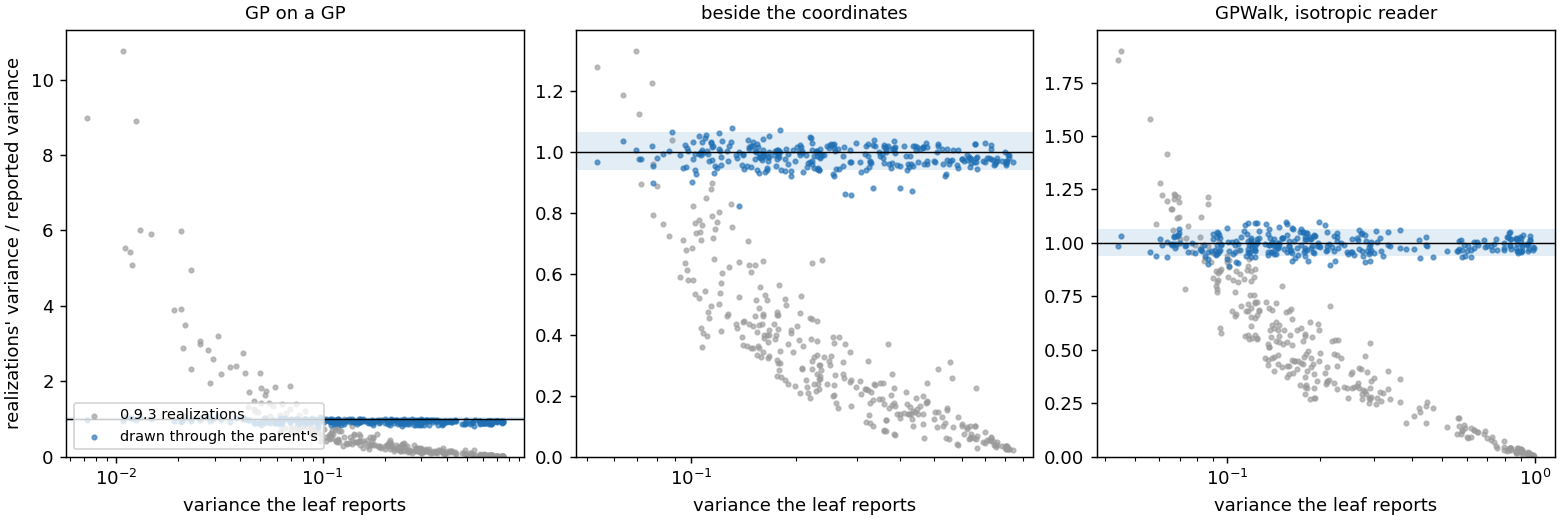
\includegraphics[width=\textwidth]{figures/gate_realizations_experts3.png}
\caption{Gate 2a with three experts: realized over reported variance per point.}
\end{figure}

\begin{figure}[h]
\centering
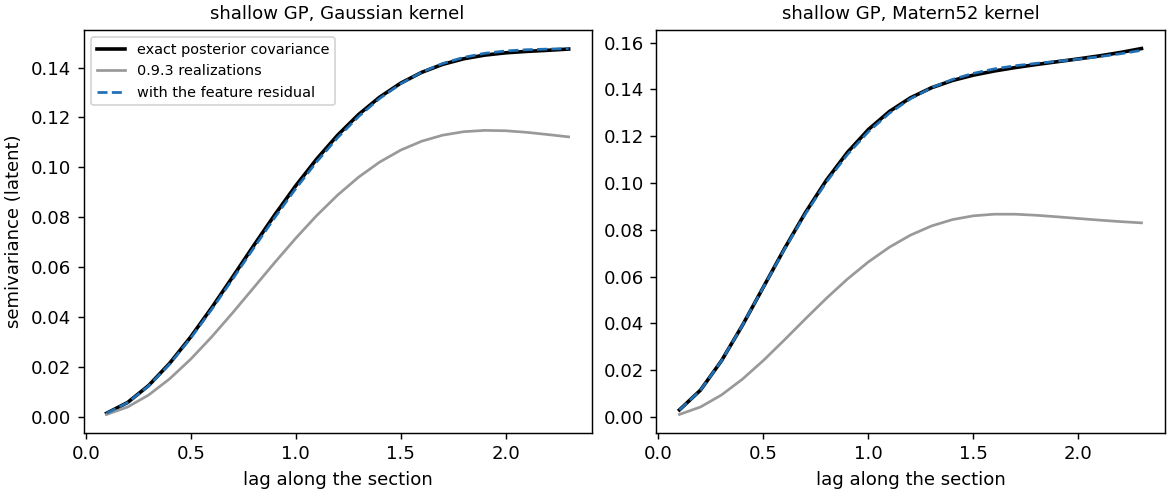
\includegraphics[width=0.85\textwidth]{figures/gate_residual.png}
\caption{A shallow GP's realizations against its exact posterior covariance.}
\end{figure}

\subsection{Training on the second moment}

Three seeds each; Walker scored against the exhaustive field, its fair
check being samples of a measurement (its truth carries the nugget the
model calls noise).

\begin{center}
\small
\begin{tabular}{llcccc}
\toprule
case & arm & RMSE & meas.\ CRPS & meas.\ 90\% cov. & time \\
\midrule
Walker, GP on a GP & 0.9.3 bound & 188 & 102.9 & 0.99 & 38 s \\
 & second moment & \textbf{160} & \textbf{84.9} & \textbf{0.89} & 504 s \\
Walker, beside coords & 0.9.3 bound & 174 & 91.9 & 0.96 & 43 s \\
 & second moment & \textbf{161} & \textbf{84.8} & \textbf{0.89} & 720 s \\
\bottomrule
\end{tabular}
\end{center}

On the folded section the new-hole log score went from $-9.6$ to $-11.2$
(moment bound) to $-1.9$ to $-2.4$ beside the coordinates. On chapter~16
the rock's log score moved from 0.3224 to 0.3204 on every seed, the metals
not at all, for 3.7 times the training time. A sampled warm-up added
nothing on any case.

\begin{figure}[p]
\centering
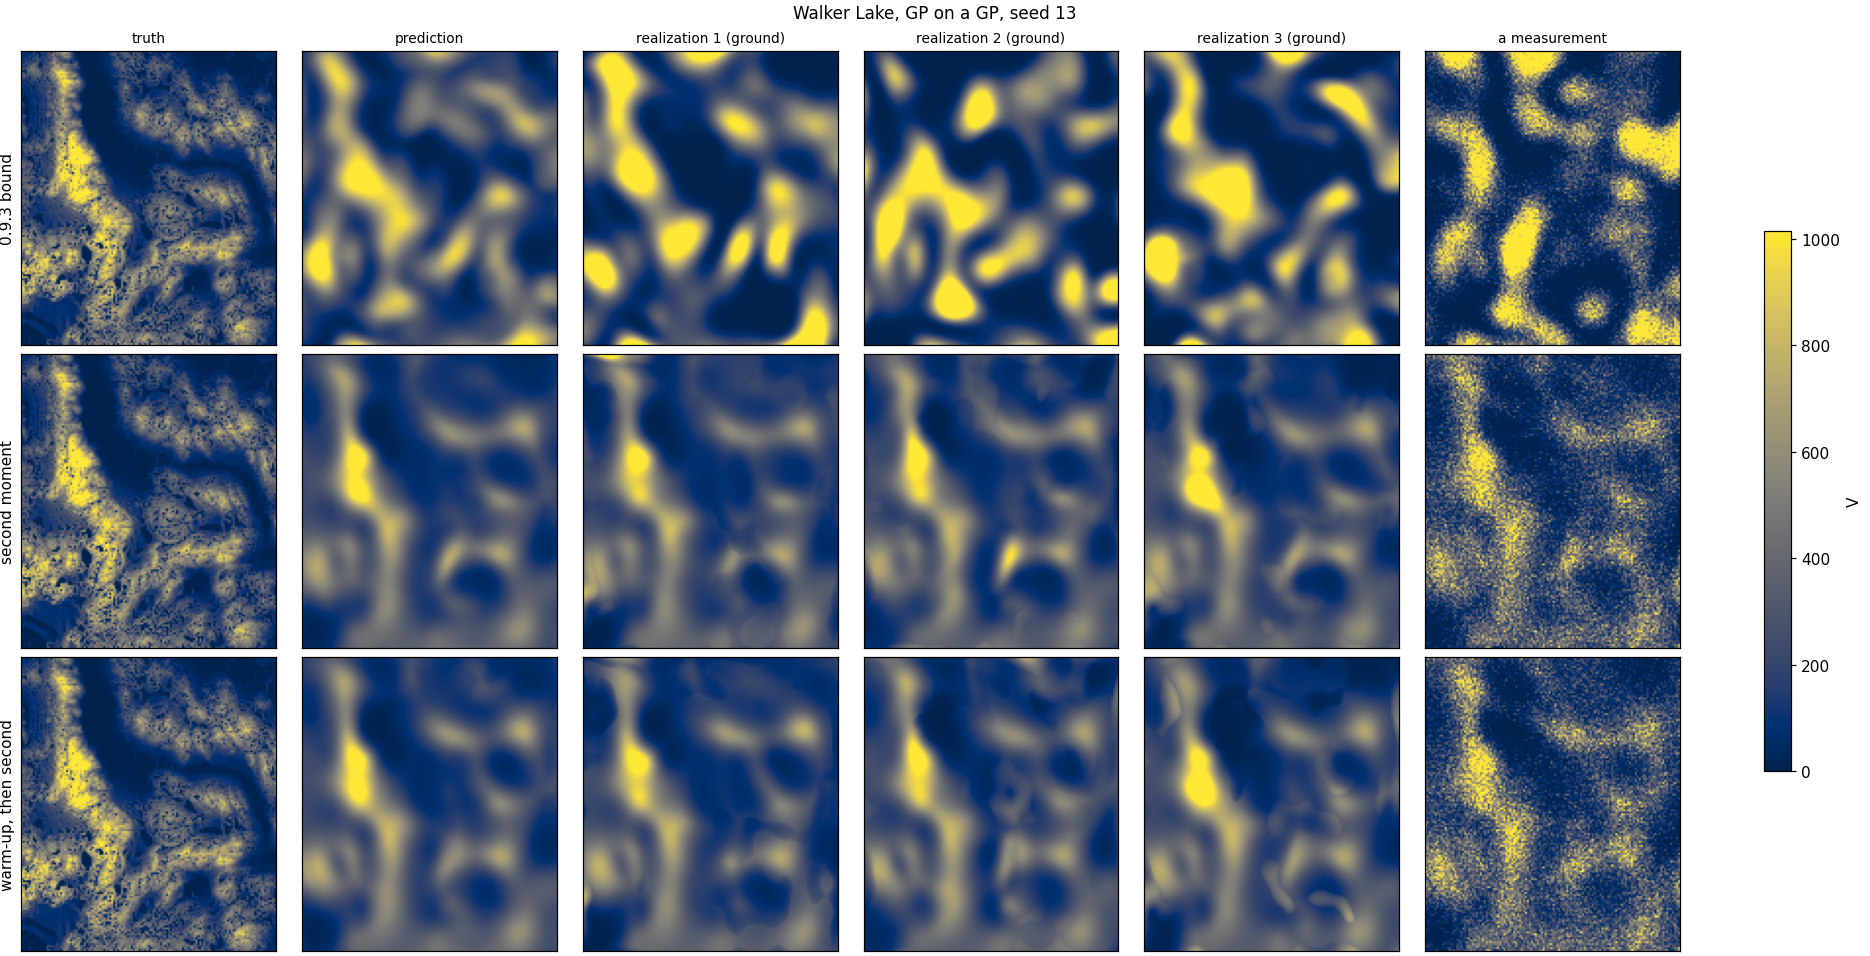
\includegraphics[width=\textwidth]{figures/phase3_walker_maps_dgp_13.png}
\caption{Walker, GP on a GP, seed 13: truth, prediction, three ground
realizations and a measurement draw, for the 0.9.3 bound (top), the
second moment (middle) and the warm-up (bottom).}
\end{figure}

\begin{figure}[p]
\centering
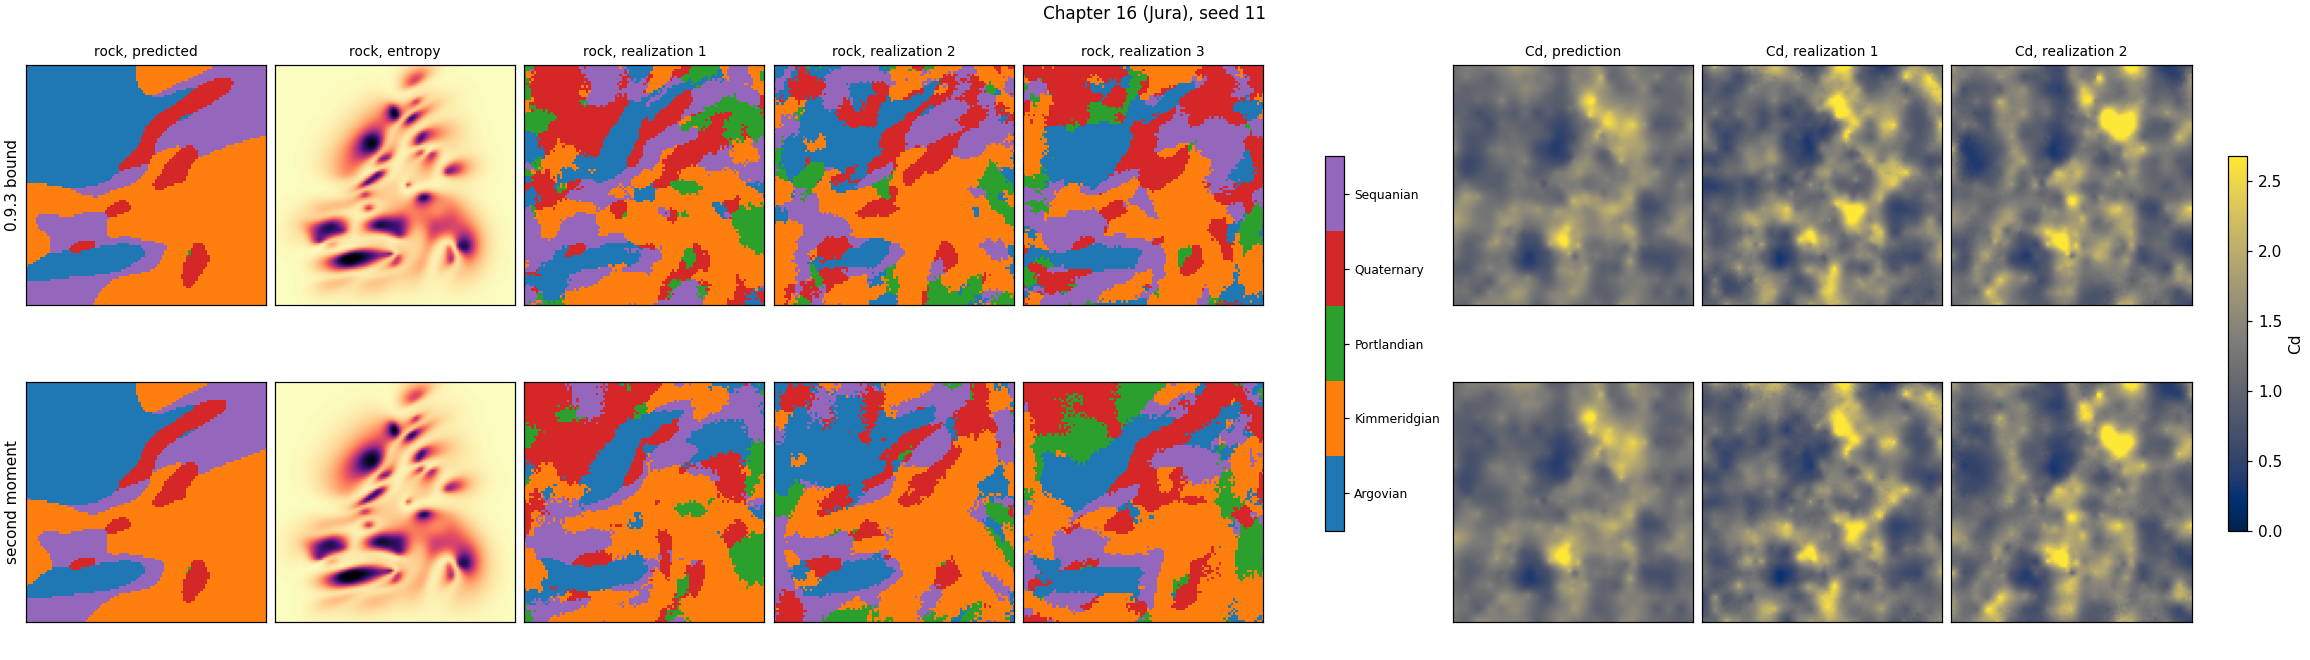
\includegraphics[width=\textwidth]{figures/phase3_jura_maps_11.png}
\caption{Chapter 16, seed 11: the rock and Cd, the 0.9.3 bound (top)
against the second moment (bottom).}
\end{figure}

\subsection{Two regressions, traced}

\paragraph{The folded ore (\code{non_stationary_test.py}).} Three
drillholes through a folded ore layer and a walked deep model at
transform range~2 folded the ore into one body in the user's 2025-09-08
copy and in commit \code{c8e4c52}, and gave five separate blobs in every
release from v0.3.5 on (three seeds each, 17 versions). Swapping v0.3.5's
files one at a time into \code{c8e4c52} put the cause in
\code{latent.py}; in it, v0.3.5 gave every GP node a trainable bias
$b\in[-5,5]$, the prior mean, which had been zero. With zero mean a field
returns to zero --- the ore/waste boundary --- away from the data, and only
a fold explains the logs; with a free bias it returns to ``waste'', and
five blobs explain them at a better bound ($-48.3$ against $-51.4$).
Fixing every bias at zero brings the fold back on v0.3.5, v0.8.8, v0.9.3
and the branch, on all three seeds; at v0.3.5 the bounds equal the old
copy's to the digit.

\begin{figure}[h]
\centering
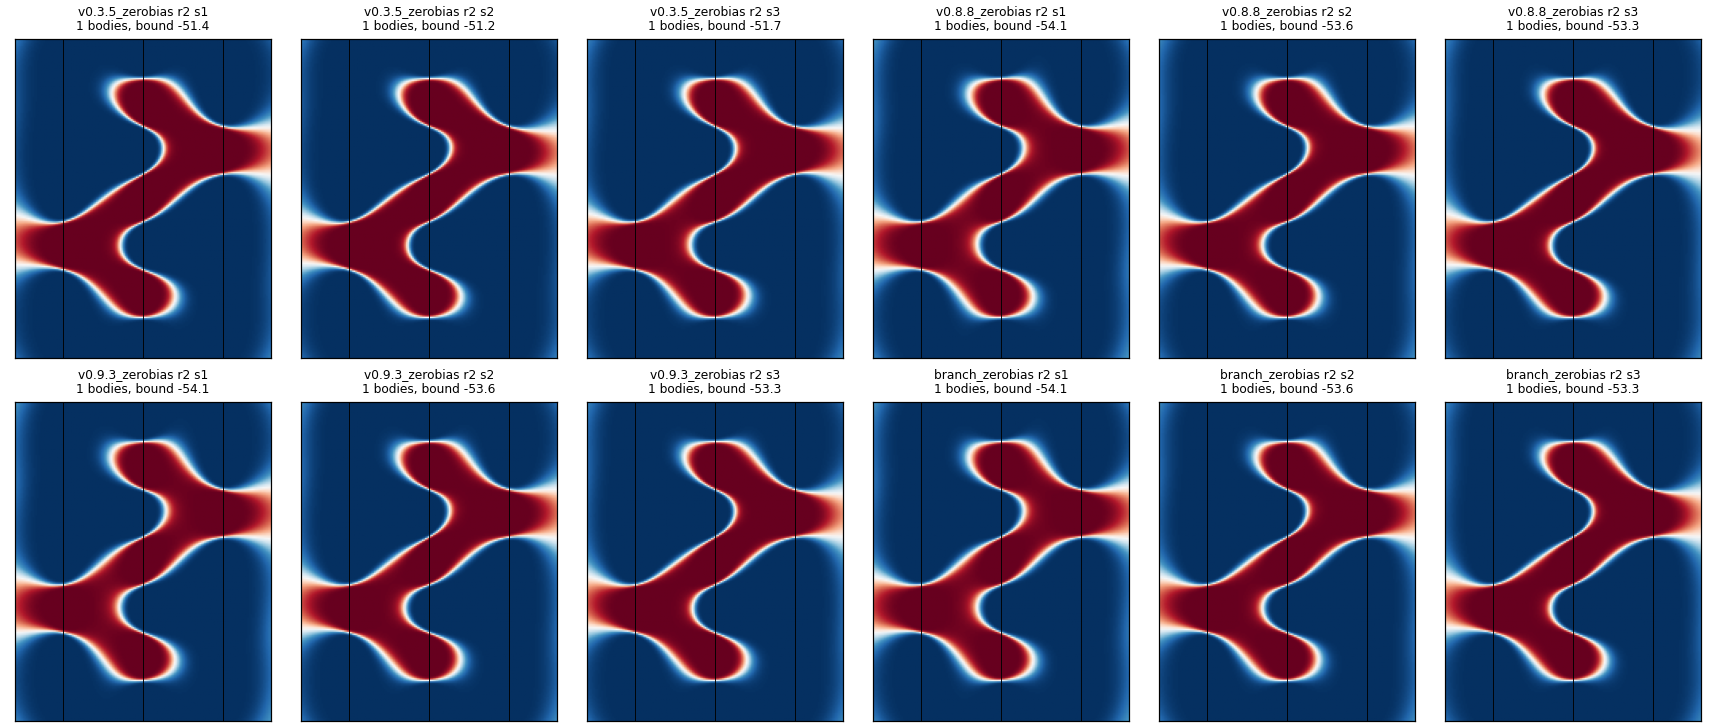
\includegraphics[width=0.75\textwidth]{figures/fold_zerobias.png}
\caption{The folded ore with every bias fixed at zero.}
\end{figure}

\paragraph{Chapter 17.} The 0.8.0 chapter's deep model is identical to
the bit from 0.8.0 to 0.8.8 and changes at 0.9.0 (bound $-1488\to-1822$,
in-sample agreement $0.983\to0.972$). Under
\code{propagation="marginal"} v0.9.3 and the branch reproduce 0.8.x to the
last digit: the change is the joint propagation made the default in
0.9.0, for which the chapter was later retuned.

\subsection{Where the time goes}\label{sec:profile}

A training step of Walker's GP on a GP is 15~ms under the moment bound
and 246~ms under the second moment on the CPU. The TF profiler puts 88\%
of the op time in the conditioned quadrature's loop --- 72\% its backward
pass, which recomputes each chunk --- on elementwise operations over
$[n,\text{chunk},m,d]$ arrays. The chunking, not the arithmetic, is much
of it:

\begin{center}
\begin{tabular}{lcc}
\toprule
quadrature, 64 nodes & CPU ms/step & GPU ms/step \\
\midrule
4 a chunk, looped (now) & 245 & 130 \\
16 a chunk, looped & 172 & 78 \\
all at once, plain autodiff & 147 & 60 \\
\bottomrule
\end{tabular}
\end{center}

\noindent (the bound identical to $10^{-8}$ in every arm). Recommended:
(1) size the chunk by a memory budget and use plain differentiation when
everything fits, keeping the recomputing loop for networks whose memory
needs it (1.7$\times$ on the CPU, 2.2$\times$ on the GPU); (2) fewer nodes
in low dimension --- a $5\times5$ Gauss--Hermite grid in two dimensions
would cost 40\% of the 64 Sobol nodes, with weighted sums; not yet
measured for accuracy; (3) the prediction is dominated by the same
quadrature (the moments); the shared-prior realizations cost under a
tenth of it.

\section*{References}
\begin{itemize}\itemsep0pt
\item Girard, A., Rasmussen, C.\,E., Quiñonero-Candela, J., Murray-Smith, R. (2003). Gaussian process priors with uncertain inputs. NeurIPS.
\item Titsias, M., Lawrence, N. (2010). Bayesian Gaussian process latent variable model. AISTATS.
\item Damianou, A., Lawrence, N. (2013). Deep Gaussian processes. AISTATS.
\item Salimbeni, H., Deisenroth, M. (2017). Doubly stochastic variational inference for deep Gaussian processes. NeurIPS.
\item Rahimi, A., Recht, B. (2007). Random features for large-scale kernel machines. NeurIPS.
\item Wilson, J., Borovitskiy, V., Terenin, A., Mostowsky, P., Deisenroth, M. (2020). Efficiently sampling functions from Gaussian process posteriors. ICML.
\item Jarzynski, M., Olano, M. (2020). Hash functions for GPU rendering. JCGT 9(3).
\end{itemize}

\end{document}
